\documentclass[a4paper,12pt]{article}
\usepackage[utf8]{inputenc} 
\usepackage{amsmath}
\usepackage{xcolor}
\usepackage{graphicx}
\usepackage[citecolor=blue]{hyperref}       % Para enlaces en el documento
\usepackage{fancyhdr}
\usepackage{circuitikz}
\usepackage{amssymb}
\usepackage{animate}
\usepackage{float}
\usepackage{multirow}
\usepackage{pgfplots}
\pgfplotsset{compat=1.18}
\usepackage[a4paper, margin=1in]{geometry}
\usepackage{gensymb}
\usepackage{siunitx}
\usepackage{booktabs}
\usepackage{listings}
\usepackage{tikz}
\usetikzlibrary{shapes.geometric, arrows, positioning}

% Ajuste de la altura del encabezado
\setlength{\headheight}{76.27646pt}
\addtolength{\topmargin}{-34.27646pt}

\lstdefinestyle{mystyle}{
    language=Matlab,
    inputencoding=utf8,
    backgroundcolor=\color{black!5},
    commentstyle=\color{green!60!black},
    keywordstyle=\color{blue},
    numberstyle=\tiny\color{gray},
    stringstyle=\color{purple},
    basicstyle=\footnotesize\ttfamily,
    breaklines=true,
    captionpos=b,
    keepspaces=true,
    numbers=left,
    numbersep=5pt,
    showstringspaces=false,
}
\lstset{style=mystyle}

\setlength{\parindent}{0pt}

% Crear la portada manualmente
\begin{document}

% Desactivar la numeración de página para la portada
\thispagestyle{empty}

% Colocar las imágenes en las esquinas superiores
\begin{minipage}[t]{0.4\textwidth}
    \raggedright
    
\includegraphics[width=2cm]{image/der.png}
\end{minipage}%
\begin{minipage}[t]{0.5\textwidth}
    \raggedleft
    
\includegraphics[width=2cm]{image/izq.png}
\end{minipage}

\vspace{1cm}

\begin{center}
    \Huge{\textbf{Previo 4. Manejo de Dispositivos de Interconectividad, hub y switch.}} \\
    \vspace{2cm}
    \Large{\textbf{Universidad Nacional Autónoma de México.}}\\
    \Large{\textbf{Facultad de Ingeniería.}}\\
    \vspace{1cm}
    \Large{Laboratorio de Redes de datos seguras.} \\
    \vspace{0.5cm}
    \LARGE{\textbf{Profesora:}}
    \LARGE{\textit{MTRA. MARIA EUGENIA BAUTISTA GONZALEZ.}}\\
    \vspace{0.5cm}
    \Large{\textbf{Grupo:} 08} \\
    \vspace{0.5cm}
    \LARGE{\textbf{Alumno:}}\\
    \Large{32006082-9} \\
    \vspace{3cm}
    \Large{\textbf{Fecha de Entrega:}}\\
    \vspace{0.5cm}
    \large{{Marzo 5, 2026}}
\end{center} 


\newpage

% Configuración del encabezado y pie de página
\pagestyle{fancy}
\fancyhf{}
\fancyhead[L]{
\includegraphics[width=1.5cm]{image/izq.png}}
\fancyhead[R]{
\includegraphics[width=1.5cm]{image/der.png}}
\fancyfoot[C]{\thepage}  % Coloca el número de página en el centro del pie de página

% Línea horizontal en el pie de página
\renewcommand{\footrulewidth}{0.4pt}  % Define el grosor de la línea en el pie de página

% Empezar numeración de páginas desde 1 en la segunda página
\pagenumbering{arabic}
\setcounter{page}{1}

%\maketitle
\tableofcontents


\newpage

\section{Realice una tabla comparativa que contenga al menos cinco características de un hub y un switch.}

El diseño y despliegue de infraestructuras de redes de área local (LAN) ha evolucionado significativamente, marcando una transición desde arquitecturas lógicas compartidas hacia topologías altamente segmentadas y gestionadas. En el epicentro de esta evolución se encuentra la distinción operativa entre los concentradores (hubs) y los conmutadores (switches). Aunque históricamente ambos dispositivos compartían la finalidad de interconectar múltiples nodos terminales, sus mecanismos de procesamiento de señales, capacidades de aislamiento de tráfico y perfiles de seguridad divergen de manera fundamental. A continuación, se presenta una tabla comparativa exhaustiva que delimita las características técnicas de ambos dispositivos.

\begin{table}[H]
    \centering
    \renewcommand{\arraystretch}{1.5}
    \begin{tabular}{|p{3.5cm}|p{5.5cm}|p{5.5cm}|}
        \hline
        \textbf{Característica} & \textbf{Concentrador (Hub)} & \textbf{Conmutador (Switch)} \\ \hline
        \textbf{Capa del Modelo OSI} & Opera exclusivamente en la Capa 1 (Capa Física). Procesa señales eléctricas en bruto. & Opera primordialmente en la Capa 2 (Enlace de Datos) y modelos avanzados en la Capa 3 (Red). \\ \hline
        \textbf{Mecanismo de Reenvío} & Inundación (Broadcast). Replica y transmite los bits recibidos por todos los puertos activos, excepto el de origen. & Reenvío inteligente (Unicast). Lee la dirección MAC de destino y envía la trama únicamente al puerto correspondiente. \\ \hline
        \textbf{Gestión de Dominios de Colisión} & Constituye un único dominio de colisión. Todos los nodos conectados compiten por el mismo medio de transmisión. & Microsegmentación. Cada puerto del conmutador establece un dominio de colisión independiente y aislado. \\ \hline
        \textbf{Asignación de Ancho de Banda} & El ancho de banda total se divide y comparte equitativamente entre todos los dispositivos activos en la red. & Ancho de banda dedicado. Cada puerto dispone de la totalidad del ancho de banda especificado (ej. 1 Gbps íntegro). \\ \hline
        \textbf{Modo de Transmisión} & Restringido a comunicación semidúplex (Half-duplex); no puede enviar y recibir simultáneamente. & Capacidad nativa de comunicación dúplex completo (Full-duplex), transmitiendo y recibiendo simultáneamente. \\ \hline
        \textbf{Tratamiento de Direcciones MAC} & Carece de memoria o inteligencia algorítmica; ignora completamente las direcciones físicas de las tramas. & Construye y mantiene dinámicamente una tabla CAM (Content Addressable Memory) para asociar MACs con puertos físicos. \\ \hline
        \textbf{Postura de Seguridad} & Altamente vulnerable. Facilita la interceptación pasiva (sniffing), ya que todo el tráfico llega a todas las interfaces. & Mayor seguridad nativa. El tráfico aislado mitiga el sniffing directo, requiriendo técnicas activas como ARP Spoofing para interceptar. \\ \hline
    \end{tabular}
    \caption{Comparativa técnica exhaustiva entre un Hub y un Switch.}
\end{table}

El análisis de estas divergencias revela que el hub funciona como un mero repetidor multipuerto pasivo. Su incapacidad para inspeccionar las tramas de datos provoca que las colisiones electromagnéticas sean una constante ineludible bajo cargas de tráfico moderadas a altas, lo que degrada drásticamente el rendimiento de la red y expone información confidencial a cualquier nodo conectado \cite{stallings2014}. 

Por el contrario, el conmutador introduce la noción de inteligencia en el borde de la red. Mediante el uso de circuitos integrados de aplicación específica (ASIC), el switch examina la cabecera Ethernet de cada trama entrante, extrae la dirección MAC de origen para poblar su tabla CAM y evalúa la dirección MAC de destino para tomar una decisión de conmutación exacta. Este paradigma de conmutación basada en hardware permite la creación de circuitos virtuales transitorios entre el emisor y el receptor, erradicando las colisiones y permitiendo que protocolos superiores operen con una latencia minimizada y un rendimiento predecible \cite{kurose2017}.


\section{¿Cómo funciona el método de CSMA/CD?}

El método de Acceso Múltiple con Detección de Portadora y Detección de Colisiones (CSMA/CD, por sus siglas en inglés: \textit{Carrier Sense Multiple Access with Collision Detection}) es un protocolo de control de acceso al medio especificado históricamente en el estándar IEEE 802.3. Su propósito fundamental es gobernar de manera probabilística el acceso equitativo a un medio de transmisión compartido, mitigando la corrupción de datos generada cuando múltiples estaciones intentan inyectar señales electromagnéticas de manera concurrente \cite{ieee8023}.

El funcionamiento operativo de CSMA/CD se estructura en una secuencia algorítmica de fases rigurosas de escucha, transmisión, detección y resolución matemática de conflictos:

En primera instancia, el mecanismo opera bajo el principio de \textbf{Detección de Portadora (Carrier Sense)}. Antes de que una interfaz de red (NIC) inicie la transmisión de una trama, debe monitorizar pasivamente el estado eléctrico o luminoso del canal de comunicaciones. Si el hardware detecta actividad (una portadora), concluye que el medio está ocupado y difiere su transmisión. Dependiendo del diseño de persistencia (usualmente 1-persistente en Ethernet), el dispositivo continuará "escuchando" ininterrumpidamente hasta que el medio quede libre. Una vez inactivo, la estación espera un intervalo temporal de guarda mínimo, conocido como \textit{Interframe Gap} (IFG), que equivale a 9.6 microsegundos en redes de 10 Mbps, antes de comenzar a emitir \cite{tanenbaum2021}.

Simultáneamente a la \textbf{Transmisión}, el protocolo activa su fase de \textbf{Detección de Colisiones (Collision Detection)}. Mientras la estación transmite, su hardware analógico compara continuamente el voltaje de la señal que está inyectando en el cable con el voltaje que percibe del mismo. Si otra estación, por latencia de propagación, asumió erróneamente que el medio estaba libre y comenzó a transmitir, las señales chocarán, provocando una superposición de ondas que eleva el nivel de voltaje más allá del umbral normal de una sola estación. El dispositivo transmisor identifica inmediatamente esta anomalía física como una colisión \cite{stallings2014}.

Al confirmar la colisión, se interrumpe inmediatamente el envío de la trama original de datos útiles. En su lugar, el nodo transmite una secuencia específica de 32 bits denominada \textbf{Señal de Atasco (Jam Signal)}. Esta ráfaga de ruido deliberado asegura que la anomalía se propague con suficiente duración para que todos los demás nodos conectados en el dominio de colisión reconozcan inequívocamente que la trama actual ha sido corrompida y debe ser descartada de sus búferes de recepción.

Finalmente, para evitar que las estaciones involucradas colisionen repetidamente al intentar retransmitir de inmediato, el protocolo invoca el \textbf{Algoritmo de Retroceso Exponencial Binario Truncado (Truncated Binary Exponential Backoff)}. Este modelo matemático descentralizado calcula un tiempo de espera aleatorio ($T_w$) antes del próximo intento de transmisión. El tiempo de espera se define como:

\

Donde el $\text{slot time}$ representa el tiempo necesario para transmitir 512 bits (aproximadamente 51.2 microsegundos en redes de 10 Mbps), y el multiplicador $r$ es un número entero aleatorio seleccionado de una distribución uniforme en el intervalo $[0, 2^k - 1]$. La variable $k$ simboliza el número de colisiones consecutivas experimentadas por esa trama. Al incrementar la ventana de probabilidad exponencialmente tras cada fallo, el algoritmo dispersa temporalmente los intentos de las estaciones, aliviando la congestión del canal \cite{kurose2017}. Si se alcanzan las 16 colisiones sucesivas, el proceso se aborta de manera definitiva y se reporta un fallo crítico a las capas superiores del modelo de red.

Cabe destacar que, en las arquitecturas modernas basadas íntegramente en conmutadores configurados en dúplex completo (Full-Duplex Gigabit Ethernet o superior), el protocolo CSMA/CD ha quedado obsoleto y desactivado por diseño, dado que la separación física de los canales de transmisión y recepción imposibilita conceptualmente las colisiones en el medio \cite{ieee8023}.

\newpage

\section{¿Qué es una colisión?}

En el contexto estricto de la ingeniería de redes de datos y telecomunicaciones, una colisión se define como un evento de interferencia destructiva que ocurre cuando dos o más dispositivos terminales intentan transmitir señales electromagnéticas o pulsos ópticos simultáneamente a través de un medio de transmisión lógico o físico compartido. Este fenómeno es característico de las topologías de red que operan en modo semidúplex (Half-duplex), tales como los sistemas basados en cable coaxial (Ethernet 10BASE2/10BASE5), conexiones mediante concentradores (hubs) o entornos inalámbricos donde el espectro radioeléctrico actúa como el medio común \cite{tanenbaum2021}.

Desde una perspectiva de la capa física, los datos se codifican mediante fluctuaciones de voltaje (en cables de cobre) o variaciones en la intensidad lumínica (en fibra). Cuando múltiples señales son inyectadas en un canal único al mismo tiempo, las ondas se superponen, sumando o restando sus amplitudes de acuerdo con las leyes de la física ondulatoria. Esta alteración eléctrica deforma irreversiblemente la codificación de la línea (como la codificación Manchester o 8b/10b). Como consecuencia, los niveles lógicos de bits ("0" y "1") se vuelven indistinguibles; la señal resultante carece de sentido semántico y se interpreta como "ruido" por las tarjetas de interfaz de red (NIC) receptoras \cite{stallings2014}. A nivel de la capa de enlace de datos, esta alteración invalida la Secuencia de Verificación de Trama (FCS), forzando a que los paquetes afectados sean irremediablemente descartados y requieran retransmisión.

La ocurrencia de colisiones está intrínsecamente ligada al \textbf{retardo de propagación} del medio. Ninguna señal viaja de manera instantánea; se desplaza a una fracción de la velocidad de la luz. Si el nodo A verifica que el medio está inactivo y comienza a transmitir, pasará una cantidad minúscula de tiempo antes de que el primer bit llegue físicamente al nodo B situado en el extremo opuesto del cable. Si durante este intervalo crítico de silencio relativo el nodo B también inicia una transmisión, se producirá una colisión en algún punto intermedio del cable. Este fenómeno dicta la longitud máxima permitida para los cables de red, garantizando que una colisión pueda propagarse de regreso al emisor antes de que termine de transmitir la trama mínima permitida \cite{kurose2017}.

Es imperativo diferenciar entre colisiones normales y \textbf{colisiones tardías (late collisions)}. Una colisión tardía es una violación crítica del protocolo en la cual la interferencia es detectada después de que la estación ya ha transmitido los primeros 512 bits (o 64 bytes) de la trama. A diferencia de las colisiones estándar, las colisiones tardías no son retransmitidas automáticamente por el hardware de la NIC, ya que suelen ser sintomáticas de graves deficiencias de diseño físico: cables que exceden los límites de longitud estipulados por el estándar IEEE, un número excesivo de repetidores en serie o una mala terminación de impedancia en el cableado \cite{ieee8023}.

La demarcación topológica donde las colisiones pueden ocurrir se denomina \textbf{dominio de colisión}. En las infraestructuras de la era temprana, toda la red constituía un solo dominio. La introducción de conmutadores (switches) y enrutadores revolucionó esta limitación al crear microsegmentaciones, donde cada puerto constituye un dominio de colisión aislado, erradicando este fenómeno en las arquitecturas empresariales contemporáneas de alta velocidad.

\newpage

\section{¿Cuál es la importancia de la capa 2 del modelo OSI?}

El modelo de Referencia de Interconexión de Sistemas Abiertos (OSI) consolida una arquitectura en siete estratos lógicos para estandarizar las funciones de los sistemas de telecomunicación. En esta jerarquía, la \textbf{Capa 2, o Capa de Enlace de Datos (Data Link Layer)}, asume una importancia crítica y cardinal: actúa como el puente traductor indispensable entre los procesos de software lógicos y abstractos de las capas superiores y las realidades físicas, caóticas y analógicas de los medios de transmisión subyacentes \cite{stallings2014}. 

La trascendencia operativa de la Capa 2 radica en su capacidad de transformar un medio de transmisión físico de la Capa 1—el cual se limita a inyectar bits en forma de flujos de voltaje o fotones crudos y propensos a interrupciones—en un canal de comunicación determinista, estructurado y libre de errores locales. Sin la intervención de la Capa 2, la red carecería de la noción de "origen" o "destino" dentro de una misma infraestructura física, y las capas superiores, como el protocolo IP en la Capa 3, se verían abrumadas intentando descifrar señales eléctricas inconsistentes \cite{tanenbaum2021}.

Para abordar esta monumental tarea de manera modular, el Instituto de Ingenieros Eléctricos y Electrónicos (IEEE), a través de su familia de estándares 802, divide estructuralmente la Capa 2 en dos subcapas especializadas:

\begin{itemize}
    \item \textbf{Control de Enlace Lógico (LLC - 802.2):} Esta subcapa superior interactúa directamente con la capa de red. El LLC es vital porque aísla a los protocolos de enrutamiento (como IPv4 o IPv6) de las especificidades del hardware. Provee mecanismos de multiplexación para que diversos protocolos de red operen simultáneamente sobre el mismo medio, además de gestionar controles de flujo rudimentarios y el acuse de recibo de tramas en servicios orientados a conexión.
    \item \textbf{Control de Acceso al Medio (MAC - 802.3/802.11):} Interactúa con la circuitería física de red. Es responsable del direccionamiento físico absoluto mediante las direcciones MAC, un identificador de 48 bits único globalmente, grabado en el hardware de la tarjeta de red (NIC). Asimismo, arbitra de manera estricta cuándo y cómo el dispositivo puede transmitir en el medio compartido (a través de protocolos de contención como CSMA/CD en ethernet heredado o CSMA/CA en Wi-Fi) \cite{kurose2017}.
\end{itemize}

Otra función cardinal que eleva la importancia de la Capa 2 es el \textbf{Control de Errores e Integridad}. La capa de enlace de datos encapsula los paquetes provenientes de la Capa 3 añadiendo un preámbulo para la sincronización de reloj, una cabecera con el direccionamiento MAC, y un remolque crucial conocido como la Secuencia de Verificación de Trama (FCS). Mediante un algoritmo de Comprobación de Redundancia Cíclica (CRC), el hardware receptor realiza una ecuación polinómica sobre el flujo de bits entrante; si el resultado difiere del hash en el FCS, se concluye que el ruido electromagnético o la interferencia ha corrompido los datos, forzando un descarte inmediato y silencioso de la trama antes de que afecte a la computadora central \cite{stallings2014}.

Desde el vector de la \textbf{Seguridad de Datos Seguros}, la Capa 2 representa la frontera perimetral inicial contra intrusiones internas. Dada la naturaleza de los protocolos de capa de enlace, amenazas periciales severas como el envenenamiento ARP (\textit{ARP Spoofing}), la suplantación de MAC (\textit{MAC Spoofing}) o la inundación de tablas CAM operan exclusivamente en esta capa, explotando la falta de validación de identidad inherente a los protocolos primigenios \cite{kurose2017}. Consecuentemente, es precisamente en la Capa 2 donde se implementan los controles de seguridad empresariales de mayor robustez contemporánea, tales como la asignación de Redes de Área Local Virtuales (VLAN, IEEE 802.1Q) para la segmentación de dominios de difusión, el protocolo IEEE 802.1X para el control de acceso a la red basado en puertos (PNAC) y la autenticación EAP, así como el protocolo MACsec (IEEE 802.1AE), que provee criptografía simétrica a velocidad de línea para garantizar confidencialidad e integridad inviolable de las tramas punto a punto \cite{ieee8023}. En síntesis, la Capa 2 no solo sostiene la topología física, sino que enarbola los cimientos de la confiabilidad y la contención de seguridad cibernética perimetral.

\newpage

\section{Describa los dos tipos de parámetros dúplex para las comunicaciones en una red Ethernet: Half dúplex y Full dúplex.}

La eficiencia del intercambio de información en las infraestructuras de telecomunicaciones Ethernet está íntimamente dictada por los parámetros de direccionalidad del flujo electromagnético del enlace, definidos mediante las configuraciones dúplex. Estos parámetros no solo gobiernan el sentido físico de la transmisión, sino que determinan la latencia subyacente y la necesidad de invocar algoritmos adicionales de control de contención. Los dos paradigmas predominantes que rigen este intercambio son el modo Semidúplex (\textit{Half-Duplex}) y el modo Dúplex Completo (\textit{Full-Duplex}).

\subsection*{Comunicación Semidúplex (Half-Duplex)}

El parámetro Half-Duplex describe un canal de comunicación de naturaleza bidireccional, pero con una restricción arquitectónica severa: el flujo de datos ocurre de forma \textbf{estrictamente alterna y secuencial}. En este entorno, una tarjeta de interfaz de red (NIC) o dispositivo de interconectividad está capacitado para transmitir información hacia un host remoto, o alternativamente, puede recibir información de dicho host; sin embargo, es electrónicamente incapaz de ejecutar ambas operaciones de transmisión y recepción al mismo instante de tiempo sobre el mismo canal lógico \cite{stallings2014}.

La analogía clásica de este paradigma es el comportamiento de los radios transmisores-receptores (walkie-talkies), donde el uso del canal de frecuencia por parte de un emisor impone obligatoriamente el silencio del nodo receptor. A nivel físico en redes Ethernet antiguas (como 10BASE-T o 100BASE-TX operando en concentradores compartidos), el modo Half-Duplex se debe a que múltiples dispositivos comparten los mismos pares de cobre o el mismo dominio de difusión base \cite{tanenbaum2021}. 

Dado que la simultaneidad de señales resulta en una interferencia eléctrica destructiva, las redes Half-Duplex dependen inexorablemente del protocolo de arbitraje CSMA/CD. En consecuencia, este modo de comunicación adolece de un rendimiento efectivo (throughput) marcadamente inferior al ancho de banda teórico etiquetado. Los requerimientos de escuchar el medio, la generación de retardos aleatorios por backoff ante colisiones, y la contienda continua por la exclusividad del cable introducen altos índices de fluctuación (jitter) y latencia predecible, lo cual perjudica las aplicaciones en tiempo real o los flujos isócronos de red \cite{kurose2017}.

\subsection*{Comunicación Dúplex Completo (Full-Duplex)}

El parámetro Full-Duplex, que hoy constituye el estándar indiscutible y obligatorio en arquitecturas modernas de conmutación empresarial, define un entorno de conectividad capaz de soportar flujos de datos bidireccionales de manera \textbf{completamente simultánea} y sin interferencias cruzadas \cite{ieee8023}. En este modelo, el canal de comunicación permite a la interfaz de red emitir paquetes de datos al mismo tiempo que los está recibiendo, análogo a una vía de autopista con carriles físicamente separados para cada sentido del tráfico o al funcionamiento de una llamada telefónica celular ininterrumpida.

Para sostener este flujo concurrente, el hardware requiere de aislamientos galvánicos y circuitería avanzada. En implementaciones de Fast Ethernet (100BASE-TX), esto se logra asignando un par de hilos trenzados dedicado en exclusiva para la transmisión (Pines 1 y 2 en conectores RJ45) y un par completamente distinto para la recepción (Pines 3 y 6). En el estándar Gigabit Ethernet (1000BASE-T), la complejidad se multiplica, ya que el hardware emplea los cuatro pares del cable UTP simultáneamente en ambas direcciones (señalización PAM-5). Para evitar colisiones internas en los mismos pares físicos, los transceptores aplican sofisticados circuitos digitales de Procesamiento de Señales Digitales (DSP) y cancelación de eco híbrido para aislar la onda transmitida de la onda recibida \cite{ieee8023}.

Las implicaciones técnicas del Full-Duplex son profundamente transformadoras para la estabilidad de la red:
\begin{enumerate}
    \item \textbf{Erradicación Definitiva de las Colisiones:} Al separar lógicamente los flujos de emisión y recepción entre puertos de switch punto a punto, la superposición de datos es físicamente imposible. Por lo tanto, el protocolo CSMA/CD se desactiva permanentemente en las tarjetas de red \cite{tanenbaum2021}.
    \item \textbf{Incremento del Ancho de Banda Teórico:} El rendimiento bidireccional efectivo del canal se duplica algorítmicamente. Un enlace Gigabit configurado operativamente en Full-Duplex provee una canalización agregada de 2 Gbps (1000 Mbps de subida garantizada independientes de 1000 Mbps de bajada), lo que optimiza exponencialmente la transferencia masiva en infraestructuras troncales de \textit{data center} y esquemas convergentes SAN/LAN \cite{stallings2014}.
\end{enumerate}

\newpage

\section{Investigue cómo es una conexión en cascada. Realice un diagrama y mencione las características de esta conexión, así como su funcionamiento.}

La \textbf{conexión en cascada (Switch Cascading)} representa la metodología de interconexión topológica más elemental y ampliamente desplegada para expandir la cobertura geográfica, la escalabilidad y la densidad de puertos de una red de área local empresarial. Esta configuración se basa en enlazar múltiples conmutadores físicos en una estructura serial o jerárquica de árbol, enrutando el tráfico desde los dispositivos de acceso en el borde de la red hacia el núcleo central, empleando para ello medios de transmisión estándar (cables UTP de pares trenzados o enlaces de fibra óptica) conectados mediante puertos regulares de acceso o puertos modulares de enlace ascendente (\textit{uplink}) \cite{tanenbaum2021}.

Históricamente, los puertos uplink o el uso de cables UTP cruzados eran obligatorios para comunicar puertos análogos entre dos switches. En la actualidad, la función \textbf{Auto-MDIX} (Automatic Medium-Dependent Interface Crossover) detecta electrónicamente la polaridad de las señales y reasigna los pares de transmisión y recepción internamente, permitiendo utilizar cables de conexión directa convencionales para extender la cascada \cite{kurose2017}.

\subsubsection*{Diagrama Esquemático: Topología en Cascada}

\begin{center}
\begin{tikzpicture}[
    node distance=2.5cm,
    switch/.style={rectangle, draw=blue!80!black, fill=blue!10, very thick, minimum width=3cm, minimum height=1.2cm, align=center, font=\sffamily\small\bfseries},
    conn/.style={ultra thick, draw=black!70, <->},
    label/.style={font=\scriptsize, color=black!80}
]
    % Core layer
    \node[switch] (core) {Switch de Distribución \\ / Núcleo (Agregador)};
    
    % First layer of cascade
    \node[switch] (acc1) [below left of=core, xshift=-3cm, yshift=-1.5cm] {Switch Acceso 1 \\ (Armario Piso 1)};
    \node[switch] (acc2) [below right of=core, xshift=3cm, yshift=-1.5cm] {Switch Acceso 2 \\ (Armario Piso 2)};
    
    % Second layer of cascade (deep cascade)
    \node[switch] (subacc1) [below of=acc1, yshift=-1cm] {Switch Acceso 1.1 \\ (Expansión Oficina)};
    
    % Connections
    \draw[conn] (core.south) -- node[sloped, above, label] {Uplink Troncal (Ej. 10 Gbps)} (acc1.north);
    \draw[conn] (core.south) -- node[sloped, above, label] {Uplink Troncal (Ej. 10 Gbps)} (acc2.north);
    \draw[conn] (acc1.south) -- node[right, label] {Cable Cobre/Cascada (Ej. 1 Gbps)} (subacc1.north);

    % Small end devices to show function
    \node[circle, fill=gray!30, inner sep=2pt, font=\tiny] (pc1) [below left of=subacc1, xshift=1cm] {PC 1};
    \node[circle, fill=gray!30, inner sep=2pt, font=\tiny] (pc2) [below right of=subacc1, xshift=-1cm] {PC 2};
    \draw[->, thick, gray] (subacc1) -- (pc1);
    \draw[->, thick, gray] (subacc1) -- (pc2);

\end{tikzpicture}
\end{center}

\subsubsection*{Características Operativas y Análisis de Funcionamiento}

El funcionamiento de una infraestructura en cascada se sustenta en el principio de independencia administrativa. Cada conmutador agregado a la cadena conserva absoluta autonomía en su \textbf{plano de control y gestión} \cite{kurose2017}. En términos de configuración técnica, esto implica que si la topología está compuesta por diez conmutadores enlazados en serie, el administrador de red debe asignar diez direcciones IP de gestión separadas, mantener diez archivos de configuración lógicos distintos, y propagar de manera manual (o mediante VTP/802.1Q) las políticas de Redes Virtuales (VLAN) de un nodo al siguiente.

Entre las características técnicas fundamentales que dictaminan el comportamiento de esta topología se encuentran:

\begin{itemize}
    \item \textbf{Gestión Descentralizada:} A diferencia de otras infraestructuras, la cascada no consolida los equipos. Carece de una dirección IP unificada, incrementando exponencialmente los costos operativos (OPEX) y la complejidad para auditorías de seguridad, actualizaciones de \textit{firmware} y monitorización SNMP, ya que cada equipo representa una entidad lógica insular \cite{stallings2014}.
    \item \textbf{Cuellos de Botella y Sobresuscripción:} El enrutamiento de flujos de datos a través de una cascada seriada impone penalizaciones de rendimiento geométricas severas. Todo el tráfico originado por decenas de puertos de host en el conmutador final (ej. Switch Acceso 1.1) debe canalizarse y converger invariablemente a través de un único puerto Ethernet en dirección hacia el núcleo de distribución. Si los enlaces ascendentes no cuentan con un diseño de sobre-aprovisionamiento masivo de ancho de banda (mediante fibras de alta densidad u óptica de 40G/100G), la red colapsará bajo su propia densidad de transmisión debido a altas tasas de contienda y sobre-suscripción (oversubscription ratios) que agotan los búferes y derivan en pérdida de tramas indiscriminada \cite{tanenbaum2021}.
    \item \textbf{Vulnerabilidad de Topología (Puntos Únicos de Fallo):} La linealidad del enlace en cascada genera fragilidades arquitectónicas inherentes. Si un conmutador intermedio dentro de la estructura sufre un fallo de hardware catastrófico o si un cable de enlace se cercena, la totalidad de los switches de las capas lógicas inferiores perderán inmediatamente toda conectividad hacia la infraestructura central \cite{kurose2017}.
    \item \textbf{Dependencia del Protocolo de Árbol de Expansión (STP):} Para mitigar las desconexiones críticas provocadas por estos Puntos Únicos de Fallo (SPOF), los ingenieros de red están forzados a implementar bucles físicos de redundancia (conectando el último switch de nuevo al núcleo principal). Esta geometría circular detona tormentas de difusión masiva (broadcast storms) que paralizarían la electrónica de procesamiento, obligando al sistema a ejecutar permanentemente el algoritmo \textit{Spanning Tree Protocol} (IEEE 802.1D / 802.1w) para mantener bloqueados lógicamente los enlaces de redundancia, mermando el ancho de banda efectivo y prolongando los tiempos de convergencia al oscilar la red ante caídas intermitentes \cite{ieee8023}.
\end{itemize}

En síntesis, la conectividad por cascada es un vector excepcionalmente rentable, ubicuo y universalmente compatible mediante cableado estándar, idóneo para despliegues de oficinas medianas. Sin embargo, su despliegue masivo lineal en redes de datos seguras empresariales de grado corporativo debe ser minuciosamente planeado o sustituido por soluciones convergentes para evadir la sofocación del throughput y la fragmentación administrativa.

\newpage

\section{Investigue cómo es una conexión en apilamiento. Realice un diagrama y mencione las características de esta conexión, así como su funcionamiento.}

La \textbf{conexión en apilamiento (Switch Stacking)} constituye el pináculo de la escalabilidad física convergente y la redundancia operativa en el diseño de redes conmutadas de alta disponibilidad de capa de acceso y distribución. Lejos de ser una mera interconexión a través de protocolos de tránsito estándar como en el escenario de la cascada, el apilamiento es una tecnología orientada por \textit{hardware y firmware propietario especializado} (por ejemplo, Cisco StackWise, FlexStack o Juniper Virtual Chassis) que permite fusionar topológicamente múltiples conmutadores físicos independientes en una amalgama simbiótica y singular, actuando funcionalmente y presentándose a la red lógica como \textbf{una única entidad o dispositivo conmutador holístico} \cite{stallings2014}.

A nivel material, los switches compatibles para stack no emplean interfaces de red frontales Ethernet comunes. En su lugar, se interconectan mediante módulos insertables en la parte trasera del chasis utilizando cables de latencia ultrabaja y ancho de banda extremo, forjando un \textit{anillo de backplane cerrado} (closed ring) o una topología en estrella \cite{tanenbaum2021}. 

\subsubsection*{Diagrama Esquemático: Topología de Apilamiento (Stacking Ring)}

\begin{center}
\begin{tikzpicture}[
    switch/.style={rectangle, draw=green!40!black, fill=green!5, ultra thick, minimum width=6cm, minimum height=1.5cm, align=center, font=\sffamily\small},
    cable/.style={ultra thick, draw=red!80!black, ->, rounded corners}
]
    % Stack Members
    \node[switch] (sw1) at (0, 0) {\textbf{Switch 1} \\ Rol: \textit{Stack Master} (Activo)};
    \node[switch] (sw2) at (0, -2.5) {\textbf{Switch 2} \\ Rol: \textit{Standby} (Espera Caliente)};
    \node[switch] (sw3) at (0, -5) {\textbf{Switch 3} \\ Rol: \textit{Miembro Base}};

    % Connectors Backplane (Right side)
    \draw[cable] (sw1.east) -- ++(1,0) |- node[midway, right, align=center, font=\scriptsize, color=black] {Anillo de Datos \\ Backplane \\ (Ej. 480 Gbps)} (sw2.east);
    \draw[cable] (sw2.east) -- ++(0.5,0) |- (sw3.east);
    
    % Ring closure (Left side)
    \draw[cable] (sw3.west) -- ++(-1.5,0) |- node[midway, left, align=center, font=\scriptsize, color=black] {Cierre de Anillo \\ Redundante} (sw1.west);

    % Logical Representation
    \draw[dashed, thick, gray] (-3, 1) rectangle (3.5, -6);
    \node[font=\sffamily\bfseries, color=gray!80!black] at (0, 1.3) {Entidad Lógica Única (Una sola Dirección IP y MAC base)};

\end{tikzpicture}
\end{center}

\subsubsection*{Características Operativas y Análisis de Funcionamiento}

La singularidad de la arquitectura de apilamiento estriba en el colapso intencionado de los planos de decisión individuales hacia un modelo de procesamiento centralizado. El funcionamiento del "stack" se fundamenta en un algoritmo electoral automatizado efectuado a nivel de sistema operativo \cite{kurose2017}. En el momento en que los dispositivos se interconectan e inicializan, se ejecutan métricas de prioridad (como nivel de \textit{hardware}, direcciones MAC más bajas o configuraciones manuales asignadas) para someter a votación un jerarca central. El sistema elegirá invariablemente un conmutador como \textbf{Maestro del Apilamiento (Stack Master)}, mientras que uno asumirá el rol de espera activa (Standby/Esclavo) y el resto actuará como miembros bases.

\begin{itemize}
    \item \textbf{Consolidación de Planos de Control y Gestión (Single Point of Management):} El funcionamiento administrativo abandona la fragmentación. El \textit{Stack Master} asimila la exclusividad absoluta de albergar las tablas de enrutamiento maestras, la memoria NVRAM del archivo general y la base de datos de control unificada de todas las interfaces. Si la pila comprende cuatro switches físicos de 48 puertos, el administrador de la red accederá mediante Telnet, SSH o SNMP a \textbf{una única dirección IP}, observando la entidad y gestionando interfaces contiguas numeradas secuencialmente (desde la interfaz 1/0/1 hasta la 4/0/48) como si constituyeran ranuras lógicas dentro de un mastodóntico y costosísimo conmutador de chasis modular \cite{stallings2014}.
    \item \textbf{Redundancia Sistémica e Intra-agregación (MEC / Failover):} Desde el punto de vista de las redes seguras y la alta disponibilidad ininterrumpida (HA), el apilamiento neutraliza catastróficos puntos únicos de fallo. Si el cable del anillo se secciona, el flujo revierte a modalidad operativa "half-bandwidth", y la comunicación continúa utilizando el anillo restante en U. Adicionalmente, si el nodo \textit{Stack Master} presenta anomalías térmicas o sufre un fallo fulminante en el circuito primario de ASIC, el sistema detona los protocolos de Convergencia de Estado Stateful Switchover (SSO) y Non-Stop Forwarding (NSF), transfiriendo en microsegundos el intelecto de control a la unidad Standby sin reiniciar interrupciones del tránsito de red inferior \cite{ieee8023}.
    \item \textbf{Abstracción Multi-Chasis y Supresión de STP:} Mientras la conexión de cascada demanda enlaces STP inactivos para prevenir desastres de enrutamiento cíclico, un diseño de Stack permite ejecutar arquitecturas formidables conocidas como Cross-Stack EtherChannel (LACP), donde cables provenientes de un servidor dual o núcleo troncal se amalgaman lógicamente a lo largo de diferentes switches físicos pero que pertenecen a un solo maestro lógico de pila. De este modo, los cables funcionan en activo-activo agregando la sumatoria de sus velocidades simultáneamente sin padecer bloqueos inducidos por el Protocolo Árbol de Expansión \cite{tanenbaum2021}.
    \item \textbf{Recursos de Conmutación de Bus y Energía Masivos:} Las matrices traseras de StackWise en arquitecturas tipo Cisco Catalyst escalan con buses ultrarrápidos permitiendo ratios de transferencia intra-switch de 320 Gbps o hasta impresionantes velocidades de magnitud Terabit (1 Tbps), anulando completamente la limitante natural de sobre-suscripción típica del cable único de la topología en cascada. Paralelamente, implementaciones especializadas extienden funciones análogas de hardware como \textit{StackPower}, lo cual entrelaza los circuitos reguladores de alimentación, distribuyendo la carga de los suministros eléctricos redundantes hacia placas físicas hermanas carentes temporalmente de flujo eléctrico local \cite{stallings2014}.
\end{itemize}

El apilamiento, aunque imperativamente restrictivo pues requiere forzosamente equipamientos idénticos de hardware de la misma serie y proveedor, personifica el diseño estándar dorado y riguroso de redes locales en la optimización corporativa presente.


\newpage

\section{¿Qué es un analizador de paquetes y cuál es su utilidad?}

En el núcleo de la administración táctica y auditoría de ciberseguridad en arquitecturas telemáticas contemporáneas, el \textbf{analizador de paquetes (Packet Sniffer, Network Analyzer o Protocol Analyzer)} actúa como el instrumento fundacional de diagnóstico heurístico y visibilidad en profundidad. Técnicamente definido, un analizador de paquetes es una aplicación de software especializada, a veces incrustada dentro de una sonda de electro-hardware distribuida, diseñada intrínsecamente para interceptar, registrar (capturar), descifrar, e interpretar a tiempo real, la totalidad de los datagramas, segmentos o tramas codificadas en binario bruto que atraviesan una capa física de red subyacente determinada \cite{kurose2017}.

Para concretar exitosamente su propósito interceptivo, el analizador ejerce una anulación selectiva temporal de los filtrados normativos estandarizados a nivel del sistema operativo huésped. En entornos Ethernet convencionales, la interfaz de red (NIC) de un ordenador está programada a nivel de silicio para acatar exclusivamente la subcapa de control de enlace MAC, descartando y omitiendo de forma automática y silente todas las ráfagas que no detenten la dirección de destino física exacta del host. El analizador de protocolos instruye al núcleo del kernel subyacente para forzar la NIC al denominado \textbf{Modo Promiscuo (Promiscuous mode)} \cite{tanenbaum2021}. Esta directiva dictamina que el adaptador fotónico o el procesador eléctrico asimile, lea y traslade a la capa de usuario la totalidad abrumadora del tráfico ajeno de broadcast, multicast e incluso unicast cruzando en las derivaciones de colisión, canalizándolo a través de bibliotecas especializadas en lenguaje C bajo nivel como *libpcap* (en sistemas Unix) o *Npcap/WinPcap* (en entornos Windows) hacia interfaces descriptivas estructuradas \cite{stallings2014}. En redes completamente conmutadas modernas (switches de topología segregada libre de colisiones), el analizador carece de eficacia por sí solo ya que los switches aíslan la información; requiere configurarse sincrónicamente en conjunto con tecnologías de infraestructura habilitando puertos de espejo, monitoreo SPAN/RSPAN (Switched Port Analyzer) o *Network Taps* ópticos divisores físicos que clonen subrepticiamente la red en ruta hacia el PC del administrador.

La \textbf{utilidad operativa e impacto crítico} de estas herramientas asume alcances panorámicos multidimensionales en ingeniería corporativa:

\begin{itemize}
    \item \textbf{Auditoría de Ciberseguridad Forense Activa y Mitigación de Vulnerabilidades:} Aporta visibilidad quirúrgica invaluable contra amenazas que atraviesan los firewalls. Al diseminar paquetes en arquitecturas, permite rastrear y confirmar si vectores de infiltración han expuesto y están exportando transacciones confidenciales sin cifrar, evidenciando contraseñas en plano viajando mediante telnet o FTP, o localizando de manera precisa los orígenes de propagación lateral subrepticia provocados por troyanos maliciosos y escaneos de Nmap indeseados en la LAN \cite{stallings2014}. 
    \item \textbf{Depuración Pericial y Resolución de Tráfico (Troubleshooting):} Constituye el recurso fundamental final al presentarse latencia indescifrable, microcortes, bucles subyacentes e inconvenientes sutiles y misteriosos de la pila TCP/IP, fallas en DHCP y peticiones a servidores de nombres (DNS). Esencialmente dota a un operador de un microscopio para desensamblar transmisiones identificando *acknowledgements* perdidos, tasas abusivas de retransmisiones (TCP Dup ACKs) debidos a conmutadores o tarjetas terminales en deficiencia que de otra forma resultarían opacos y encubiertos al nivel del usuario base \cite{kurose2017}.
    \item \textbf{Ingeniería de Software Analítica y Desarrollo de Estándares Modulares:} Son cruciales instrumentales educativos universitarios y entornos de validación experimental en la codificación y refactorización algorítmica donde desarrolladores verifican exhaustivamente al nivel de cada campo de cabecera implementada a medida, comprobando a fondo que los módulos del formato de protocolo o APIs REST interconectando estructuras respondan con conformidad a la sintaxis del modelo estandarizado rfc.
\end{itemize}



\section{Mencione otras tres herramientas de análisis de paquetes y sus características}

La industria ha consolidado ecosistemas altamente desarrollados y diversificados de recolección algorítmica. Dependiendo del alcance arquitectónico, de los rigores sobre memoria volátil u operativa computacional remota de infraestructura sin pantallas periciales GUI, tres de los pilares determinantes en la recolección de paquetes, excluyendo su definición nominal primaria, se abordan a continuación:

\subsubsection*{1. Wireshark}
Concebido originariamente bajo el designio de Ethereal y evolucionando hasta afianzarse incontrovertiblemente como la referencia de código abierto predominante de facto (estándar de la industria forense gráfica interactiva), \textbf{Wireshark} brinda un microscopio algorítmico sumamente amigable hacia el análisis relacional a profundidad y disección interactiva presencial de flujos \cite{stallings2014}.

\begin{itemize}
    \item \textbf{Inspección Caleidoscópica de Disección Profunda:} Cuenta con decodificadores (*dissectors*) soportados modularmente para desentrañar microscópicamente el ensamblaje en formato legible para miles de jerarquías de protocolos estandarizados antiguos y emergentes de capas desde IEEE 802.11 inalámbrico y BlueTooth, a flujos superiores encapsulados orientados a la red LAN e IoT.
    \item \textbf{Reglas de Color y Búsqueda Analítica Heurística Inmediata:} El entorno de panel analítico proporciona coloración basada en comportamiento estructural; los administradores identifican flujos consistentes, y errores graves intermitentes con tramas corruptas en secuencias CRC marcadas intuitivamente con colores disonantes o rojo severo, facilitando inspección sobre extensas sesiones de navegación laberíntica.
    \item \textbf{Descompresión y Desencriptación Dinámica:} Ofrece una excepcional versatilidad computacional para el peritaje decodificando ráfagas capturadas cifradas de algoritmos estandarizados simétricos, como intercepciones asimiladas sobre la marcha en esquemas WPA/WPA2 de protección Wi-Fi, ISAKMP, IPsec o túneles cifrados corporativos en SSL/TLS asumiendo el suministro legal y administrativo previo de las credenciales de llaves privadas generadas en el entorno auditado \cite{kurose2017}.
    \item \textbf{Reconstrucción e Inteligencia de Sesiones de Streaming:} Cuenta con capacidades insuperables para orquestar y re-crear transacciones visuales abstractas de extremo a extremo y diagramas lógicos direccionales, reconstruyendo métricas interactivas y reproducción acústica directa para telefonía IP digitalizada de Voz sobre protocolos (VoIP) SIP u RTP evaluando anomalías y fragmentaciones sonoras (\textit{jitter} de fluctuación de ráfagas).
\end{itemize}

\subsubsection*{2. tcpdump}
En contraste diametral con la interfaz de ventana amigable orquestada para uso escritorio de la suite anterior, \textbf{tcpdump} se posiciona estrictamente como una formidable utilidad nativa minimalista accionada exclusivamente y orientada desde terminal y línea de consola iterativa (CLI). Inseparable históricamente en la administración y robustez de servidores desplegados sobre ecosistemas hipervirtualizados puros Unix/Linux \cite{tanenbaum2021}.

\begin{itemize}
    \item \textbf{Factor de Penalización Operacional Diminuta y Minimalismo Sistémico:} La aplicación resulta ideal en intervenciones periciales en ambientes que carezcan permanentemente por naturaleza o seguridad absoluta (Data Centers y servidores Cloud de comando) de un entorno gráfico nativo de control inoperable (headless). Se asienta operando de inmediato con ínfima latencia o acaparamiento del procesador físico.
    \item \textbf{Motor Filtrador Boolean Berkely (BPF):} Utiliza un motor léxico subyacente y gramática booleana estructurada, lo cual requiere que el ingeniero redija una semántica paramétrica concisa pero tremendamente refinada en la instrucción de línea para que las librerías eliminen los vectores inútiles de congestión y capturen paquetes exclusivos destinados, por ejemplo, a un destino IP de origen específico interactuando mediante puertos específicos, todo realizado dinámicamente operando y filtrando a velocidad extrema inalterable al mismo ritmo y volumen intrínseco del canal original \cite{kurose2017}.
    \item \textbf{Exportación Silente Retardada:} Principalmente abocado a recolección volumétrica programada masiva de auditorías asincrónicas desatendidas o instrumentación continua guardada para derivar y vaciar flujos recolectados hacia contenedores de datos de estructurados legibles (extensiones y codificaciones `.pcap`), idóneos para ingestiones procesables y visualizadas con posterioridad interconectando el análisis derivado del archivo crudo con metodologías forenses gráficas como Wireshark o terminales especializadas remotas \cite{stallings2014}.
\end{itemize}

\subsubsection*{3. OmniPeek}
Elevándose arquitectónicamente sobre herramientas limitadas analíticas para escalar transversalmente como una plataforma robusta y distribuida, propietaria y licenciada orientada a arquitecturas organizacionales mastodónticas y telecomunicaciones con infraestructura pesada, se inscribe y define **OmniPeek** de LiveAction.

\begin{itemize}
    \item \textbf{Capacidades para Volúmenes Industriales Trascendentales y Fibra de Núcleo:} Sobresale instrumentalmente sobre analizadores básicos cuando es exigido al operar interconectándose directamente al procesar matrices estructurales inabarcables provenientes de conmutadores intercontinentales Ethernet operando a magnitud de banda ancha vertiginosa extrema de 40 Gbps e infraestructura de 100 Gigabits ópticos, garantizando no producir embudos ni colapsos analíticos en despliegues con cuotas masivas de paquetes por segundo \cite{stallings2014}.
    \item \textbf{Caza Prospectiva de Amenazas Remotas Orquestadas (Advanced Threat Hunting):} Incorpora sondas paramétricas operativas periféricas distribuidas asincrónicamente mediante nodos *LiveWire* esparcidos y diseminados a lo ancho de arquitecturas geográficamente separadas cruzando esquemas remotos SD-WAN. Su paradigma radica en enviar toda telemetría concentrada a nivel experto con modelados de análisis histórico de vulneraciones para conformar centros logísticos de inteligencia forense remotos, detectando alteraciones operando en tableros dinámicos.
    \item \textbf{Integración Completa con Estándares Inalámbricos Críticos Múltiples Simultáneos:} Proveedor excepcional para resolución de incidencias en densidades críticas de áreas Wi-Fi empresariales; permite monitoreos pasivos interconectando adaptadores canalizados de radiofrecuencias distribuidos para captura sincronizada sobre múltiples frecuencias y espectros canales paralelos al unísono identificando mermas imperceptibles físicas.
\end{itemize}


\section{Mencione otras tres herramientas de simulación de redes y sus características.}

La predicción y validación matemática de parámetros escalables y configuraciones arquitectónicas avanzadas subyacentes requieren modelizaciones previas libres del compromiso de recursos y riesgos en inversiones lógicas físicas. Aunque el ecosistema Cisco emplea primordialmente metodologías abstraídas educacionales (como el renombrado simulador instructivo Cisco Packet Tracer), existe un abanico analítico dispar desde infraestructuras que ejecutan software algorítmico idéntico en virtualización, hasta laboratorios matemáticos precisos dependientes de programación formal en código puro. Tres herramientas que encabezan las metodologías alternativas de modelado se exponen a continuación:

\subsubsection*{1. GNS3 (Graphical Network Simulator 3)}
Divergiendo ontológicamente de abstracciones que "imitan" de forma parcial funciones internas, \textbf{GNS3} conforma en su estricta y absoluta totalidad tecnológica un **Emulador de Redes** arquitectónico maduro profesional, cimentando entornos hiperrealistas donde se ejecuta firmware fidedigno corporativo con las complejidades formales absolutas originarias del mismo.

\begin{itemize}
    \item \textbf{Hypervisor de Firmware Real y Arquitectura de Multi-proveedor Operativa:} Al operar orquestándose subyacentemente con emuladores nativos potentes informáticos en línea de comando hipervisor (Dynamips), el usuario aprovisiona legalmente el sistema operativo e imágenes ROM originales extractadas fielmente del circuito integrado (ej. imágenes de Cisco IOS nativo, Juniper OS, enrutadores modulares VyOS, infraestructura Fortigate, y Cortafuegos de Próxima Generación o NGFW de Palo Alto). Como corolario, la computadora huésped anfitriona ejecuta la abstracción procesando idénticamente cada instrucción lógica real exigiendo en el equipo base masivas cantidades directas de RAM volátil \cite{stallings2014}.
    \item \textbf{Convergencia Práctica Directa y Sinergia Computacional Exterior:} A diferencia del encierro esquemático, GNS3 posibilita anclar interfaces conectadas de laboratorio en topología a interfaces físicas operativas LAN externas del propio hardware anfitrión integrándose con la telaraña real del planeta de comunicaciones (VLAN directas). Integra complementariamente y se entrelaza de manera automatizada a máquinas invitadas de VMware nativas (ej. incorporando nodos inyectores de penetración Kali Linux directos para ejecutar validaciones ofensivas de ciberataques) y posee llamadas funcionales instantáneas invocando interceptores con \textit{Wireshark} acoplados en su propia visualización GUI en cada interfaz creada sobre demanda \cite{kurose2017}.
\end{itemize}

\subsubsection*{2. NS-3 (Network Simulator 3)}
Instaurado fundacionalmente bajo los exigentes requerimientos del ámbito científico formal institucional académico universitario de investigación analítica avanzada e innovación pionera industrial, el modelo \textbf{ns-3} de código libre abierto emerge como el pináculo del \textbf{Simulador Secuencial Analítico Operado por Eventos Discretos}.

\begin{itemize}
    \item \textbf{Precisión Matemático-Topológica Determinista Sin Interfaz de Dibujo Abstraída:} ns-3 desecha la creación estática trivial de esquemas visuales gráficos orientados por iconografía. Por el contrario, se configura y construye obligadamente con extrema minuciosidad formal rigurosa modelizando topologías codificando y parametrizando \textit{scripts} instruccionales compilados y diseñados sintácticamente en lenguaje C++ y estructurados a base interpretada de Python \cite{tanenbaum2021}.
    \item \textbf{Emulación Operativa a Nivel de Onda Celular Avanzada (Non-IP/Wi-Fi/LTE):} La valía instrumental descollante se enfoca a evaluar modelados estáticos y dinámicos que extreman profundidades de propagación física y modelos de atenuación abstractos teóricos de antenas que aún no son estandarizados comercialmente. Posee arquitecturas integradas nativas reproduciendo algoritmos WiFi teóricos a nivel electromagnético intrínseco, parámetros 4G-LTE y WiMAX pioneros o matrices especializadas de algoritmos móviles estáticos *ad hoc* inalámbricos AODV/OLSR.
    \item \textbf{Sinergia Lógica y Temporizador Bucle Empírico Tiempo-Real:} Incorpora el soporte de un módulo de temporizador \textit{scheduler-en-tiempo-real}, posibilitando simetría empírica inyectable (*Simulation-in-the-loop*); donde su software asimila y propaga flujos de inyecciones originadas de elementos computacionales genuinos colindantes operando interactuando mediante túneles evaluando variaciones del kernel informático de una placa madre Linux en redes virtualizadas subyacentes ns-3 para pruebas matemáticas algorítmicas de retrasos (\textit{Delay}, interrupciones y ecos de ráfagas) antes de lanzar producción \cite{kurose2017}.
\end{itemize}

\subsubsection*{3. EVE-NG (Emulated Virtual Environment Next Generation)}
Instaurándose orgánicamente en años venideros para desplazar barreras corporativas sobre topologías intrincadas empresariales extensas sin dependencia hiper-compleja en un terminal, el ecosistema de emulación **EVE-NG** se presenta como un entorno colaborativo multiplataforma avanzado sin ataduras (Client-less).

\begin{itemize}
    \item \textbf{Alojamiento Basado en Servidores Bare Metal Virtualización Integral KVM:} Mientras herramientas genéricas sobrecargan limitadamente una memoria PC operando instancias nativas dispares, EVE-NG ejecuta orgánicamente sobre una arquitectura hipervisor KVM base unificada proveyendo asombrosa eficiencia operacional, operando preferiblemente dedicado a infraestructuras centralizadas escalables alojadas \textit{Bare Metal} en servidores y centros ESXi donde puede recrear sinapsis masivas y topologías multi-fabricante CCIE convergentes y uniendo múltiples tecnologías que en hardware superaría exponencialmente costes monumentales o millones invertidos en rack para licencias corporativas.
    \item \textbf{Ingreso de Flujo Asincrónico y Movilidad Vía Cliente Web-HTML5 Nativo:} Trasladó la arquitectura superando dependencias monolíticas. Prescinde drásticamente del requerimiento formal administrativo de poseer interfaces y terminales cargadas e instaladas software local del usuario; funciona mediante un paradigma colaborativo y un portal enrutado íntegramente HTML5 universal proveyendo agilidad pericial inigualable a grupos y especialistas y estudiantes sinérgicos desde el explorador donde construyen y entrelazan a nivel web los parámetros interactivos de laboratorios con accesos distribuidos por credenciales centralizadas controladas \cite{stallings2014}.
\end{itemize}


\begin{thebibliography}{9}
    
    % Kurose & Ross (Top-Down Approach, foundational for OSI, Switches, CSMA/CD, Full Duplex)
    \bibitem{kurose2017} 
    Kurose, J. F., \& Ross, K. W. (2017). \textit{Computer Networking: A Top-Down Approach} (7th ed.). Pearson.

    % Stallings (Data and Computer Comms, foundational for Hub vs Switch, Encodings, Analyzers, Hardware layers)
    \bibitem{stallings2014} 
    Stallings, W. (2014). \textit{Data and Computer Communications} (10th ed.). Pearson.

    % Tanenbaum (Computer Networks, extremely good for CSMA/CD math, collision domains, physical medium delays, Emulation vs Simulation)
    \bibitem{tanenbaum2021} 
    Tanenbaum, A. S., Feamster, N., \& Wetherall, D. J. (2021). \textit{Computer Networks} (6th ed.). Pearson.

    % IEEE Standard for Ethernet (Definitive source for MACsec, 802.3, Duplex parameters, CSMA/CD formal depreciation in GigE)
    \bibitem{ieee8023} 
    IEEE Computer Society. (2018). \textit{IEEE Standard for Ethernet (IEEE Std 802.3-2018)}. IEEE. Recuperado de \url{https://standards.ieee.org/standard/802_3-2018.html}

\end{thebibliography}

\end{document}